% !TeX root = ../main.tex

\chapter{背景知识与研究现状}\label{chap:related-work}

本章介绍与本文研究内容密切相关的背景知识和研究现状。
首先，第\ref{sec:related-tech}节介绍本文所涉及的相关背景知识，包括深度学习训练的基本原理、
大语言模型推理的关键机制以及深度强化学习的理论框架。
其次，第\ref{sec:dl-sched-survey}节和第\ref{sec:llm-sched-survey}节分别从
深度学习训练集群调度和大语言模型推理集群调度两个方向，系统梳理相关研究现状，
分析现有方法的优势与不足。最后，第\ref{sec:chap2-summary}节综合梳理现有方法的局限性，明确本文的研究切入点。

\section{背景知识}\label{sec:related-tech}

\subsection{深度学习训练基础}\label{subsec:dl-training-basics}

深度学习通过构建多层非线性变换的神经网络模型，从大规模数据中自动学习特征表示，
已在计算机视觉~\cite{krizhevsky2012imagenet,dosovitskiy2020image}、
自然语言处理~\cite{sutskever2014sequence,bahdanau2014neural}、
语音识别~\cite{hinton2012deep,chan2016listen}等领域取得了突破性进展。
本节介绍深度学习模型的分布式训练机制以及弹性训练技术，
为第三章中涉及的GPU集群调度问题提供必要的技术背景。

%\textbf{模型训练基本流程。}
%深度学习模型的训练过程本质上是一个基于梯度下降的迭代优化过程\cite{}。
%在每一次训练迭代中，模型首先执行前向传播：将一个批次（mini-batch）的训练样本输入网络，
%逐层计算各层的激活值，最终得到模型的预测输出。随后，通过损失函数度量预测输出与真实标签之间的偏差，
%得到当前迭代的损失值。在此基础上，模型执行反向传播：利用链式法则从输出层向输入层逐层计算损失函数
%关于各层参数的梯度。最后，优化器（如随机梯度下降SGD\cite{}或Adam\cite{}）根据计算得到的梯度更新模型参数，
%以降低损失函数值。上述前向传播、反向传播与参数更新三个阶段构成一次完整的训练迭代，
%模型通过反复执行大量迭代逐步收敛至最优或近最优解。

\textbf{数据并行训练。}
随着模型规模和训练数据量的持续增长，单个GPU的计算能力和显存容量往往
难以满足训练需求，分布式训练已成为加速深度学习模型训练的关键手段~\cite{sergeev2018horovod,li2020pytorch}。
其中，数据并行~\cite{li2014scaling}是当前最为广泛使用的分布式训练范式。
在数据并行模式下，每个参与训练的GPU（称为一个Worker）持有模型的完整副本，
训练数据则被均匀划分为若干子集并分配给各个Worker。在单次迭代中，各Worker独立地对其子集数据
执行前向传播和反向传播以计算本地梯度，随后通过集合通信操作（如All-Reduce~\cite{thakur2005optimization, sergeev2018horovod}）
在所有Worker之间同步梯度，确保各Worker上的模型参数保持一致。
同步完成后，各Worker使用聚合后的梯度独立更新本地模型参数。
数据并行的核心优势在于可以通过增加Worker数量来等比例扩大每次迭代的有效批次大小，从而提升训练吞吐量。

\textbf{弹性训练与检查点机制。}
在多租户GPU集群环境中，可用资源随时间动态变化。弹性训练~\cite{li2020pytorch}允许训练任务在工作节点数量发生动态变化（扩容或缩容）时，
无需终止进程即可自适应地重新协调训练配置，继续执行。在调度器介入执行资源重分配的场景下，
训练任务可通过检查点（Checkpoint）机制持久化当前训练状态（包括模型参数、优化器状态及训练进度），
并在获得新资源分配后从最近的检查点无缝恢复执行。
这种机制使得调度器能够在每个调度轮次对全部GPU资源进行统一调配，
根据任务的最新训练进度和优先级动态调整资源分配方案，从而提升集群整体的资源利用率~\cite{peng2018optimus,qiao2021pollux}。

%\textbf{训练吞吐量与扩展效率。}
%训练吞吐量通常定义为单位时间内模型可执行的训练迭代次数（iterations/s）或处理的样本数量（samples/s），
%是衡量训练任务资源利用效率的核心指标\cite{}。在数据并行训练中，
%当Worker数量增加时，虽然单次迭代的有效批次大小线性增长，但训练吞吐量的提升
%通常呈现亚线性的非线性关系。这一现象的主要原因包括：
%梯度同步引入的通信开销随Worker数量的增加而增大\cite{}；
%跨节点通信的延迟通常高于节点内通信；
%此外，过大的批次大小可能导致模型收敛速度减缓，需要更多的迭代才能达到相同的性能水平\cite{}。
%上述非线性扩展特性使得为训练任务确定最优的GPU分配数量成为一个非平凡的决策问题，
%也是集群调度器需要重点优化的目标之一。

\subsection{大语言模型推理基础}\label{subsec:llm-inference-basics}

大语言模型（Large Language Model, LLM）~\cite{brown2020language}
是基于Transformer架构构建的大规模自回归语言模型，其通过在海量文本语料上进行预训练，获得了强大的自然语言理解
与生成能力。
本节介绍LLM推理服务的核心机制，为第\ref{chap:agent-routing}章涉及的LLM推理服务调度问题提供技术背景。

\textbf{LLM推理引擎核心机制。}
LLM的推理过程采用自回归生成方式，即模型每次仅生成一个输出token，
并将该token追加到已有序列中作为下一步的输入，随后模型反复执行上述过程直至生成终止标记或达到最大长度限制。
这一过程可分为两个阶段：预填充阶段（Prefill）和解码阶段（Decode）。
在预填充阶段，模型并行计算用户输入的完整提示（Prompt），并生成所有输入token对应的
中间表示以及第一个输出token；在解码阶段，模型逐个生成后续的输出token，
每一步仅依赖最新生成的单个token进行计算。由于预填充阶段涉及对整个输入序列的并行计算，
其计算开销通常远大于单步解码阶段，但解码阶段的总延迟取决于生成token的数量，
因此在输出序列长度显著大于输入长度的典型交互式应用场景中，
解码阶段的累积延迟往往占端到端推理总延迟的主要部分；
而当输入上下文极长时，预填充阶段的计算开销则可能成为延迟瓶颈。

为提升推理引擎的显存管理效率，PagedAttention~\cite{kwon2023efficient}借鉴操作系统的虚拟内存分页思想，
将键值缓存（KV Cache）划分为固定大小的物理块，通过块表（Block Table）建立逻辑页到物理块的映射，
从而实现非连续的显存分配与动态扩展。该机制显著提升了显存利用率，使推理系统能够支持更多并发请求。
在批处理策略方面，传统的静态批处理要求同一批次中的所有请求同时开始、同时结束，
导致短请求完成后需等待长请求，造成GPU资源的严重浪费。
连续批处理（Continuous Batching）~\cite{yu2022orca}机制允许在每次迭代后动态地将已完成的请求移出批次，
并将新到达的请求加入批次，从而大幅提升GPU的计算利用率。
当前主流的LLM推理引擎（如vLLM~\cite{kwon2023efficient}和SGLang~\cite{zheng2024sglang}）均采用了上述技术，
并在此基础上实现了迭代级调度，
即推理引擎在每次前向传播迭代后都可以重新组织批次中的请求，进一步优化系统的资源利用率。


\textbf{键值缓存机制与前缀缓存复用。}
在Transformer的自注意力计算中，每个token需要与序列中所有前序token的
Key和Value向量进行交互。若在解码阶段的每一步都对整个序列重新计算所有历史token的Key和Value，
将引入大量冗余计算开销。为此，在Transformer自注意力机制\cite{vaswani2017attention}的基础上，
现代大语言模型推理系统普遍采用键值缓存机制\cite{yu2022orca,kwon2023efficient}：
该机制通过缓存历史token的Key和Value向量，使得解码阶段每一步的注意力计算复杂度从
$O\left(n^2\right)$（无缓存时需重新计算所有历史token的K/V向量并执行全序列注意力）降低至
$O\left(n\right)$（$n$为当前序列长度），即每步仅需计算新token与已缓存K/V的注意力，
显著提升了自回归解码的推理效率。
然而，键值缓存的显存占用与序列长度和并发请求数量成正比，在高并发场景下，
GPU显存容量往往成为制约系统吞吐量的关键瓶颈。

在前缀缓存复用方面，当多个请求共享相同的前缀（如相同的系统提示词或少样本示例）时，
可以直接复用已缓存的公共前缀键值数据，避免对这部分内容的重复预填充计算，
从而显著节约计算资源与显存。vLLM~\cite{kwon2023efficient}利用自动前缀缓存（Prefix Caching）实现了历史状态的复用。
其核心机制是：将token序列的内容哈希值作为键，在全局哈希表中维护与物理键值缓存块的映射关系。
当新请求的token前缀计算出的哈希值在表中命中时，即可直接映射并复用底层现有的KV数据，
直接跳过冗余的预填充阶段。SGLang则进一步提出了基数树注意力
（RadixAttention），利用基数树（RadixTree）数据结构对系统中所有历史请求的键值缓存
进行统一索引与管理，以token序列为键实现键值缓存的细粒度前缀匹配与共享，
支持多请求并发场景下更高效的动态前缀复用。

\begin{figure}[htbp]
    \centering
    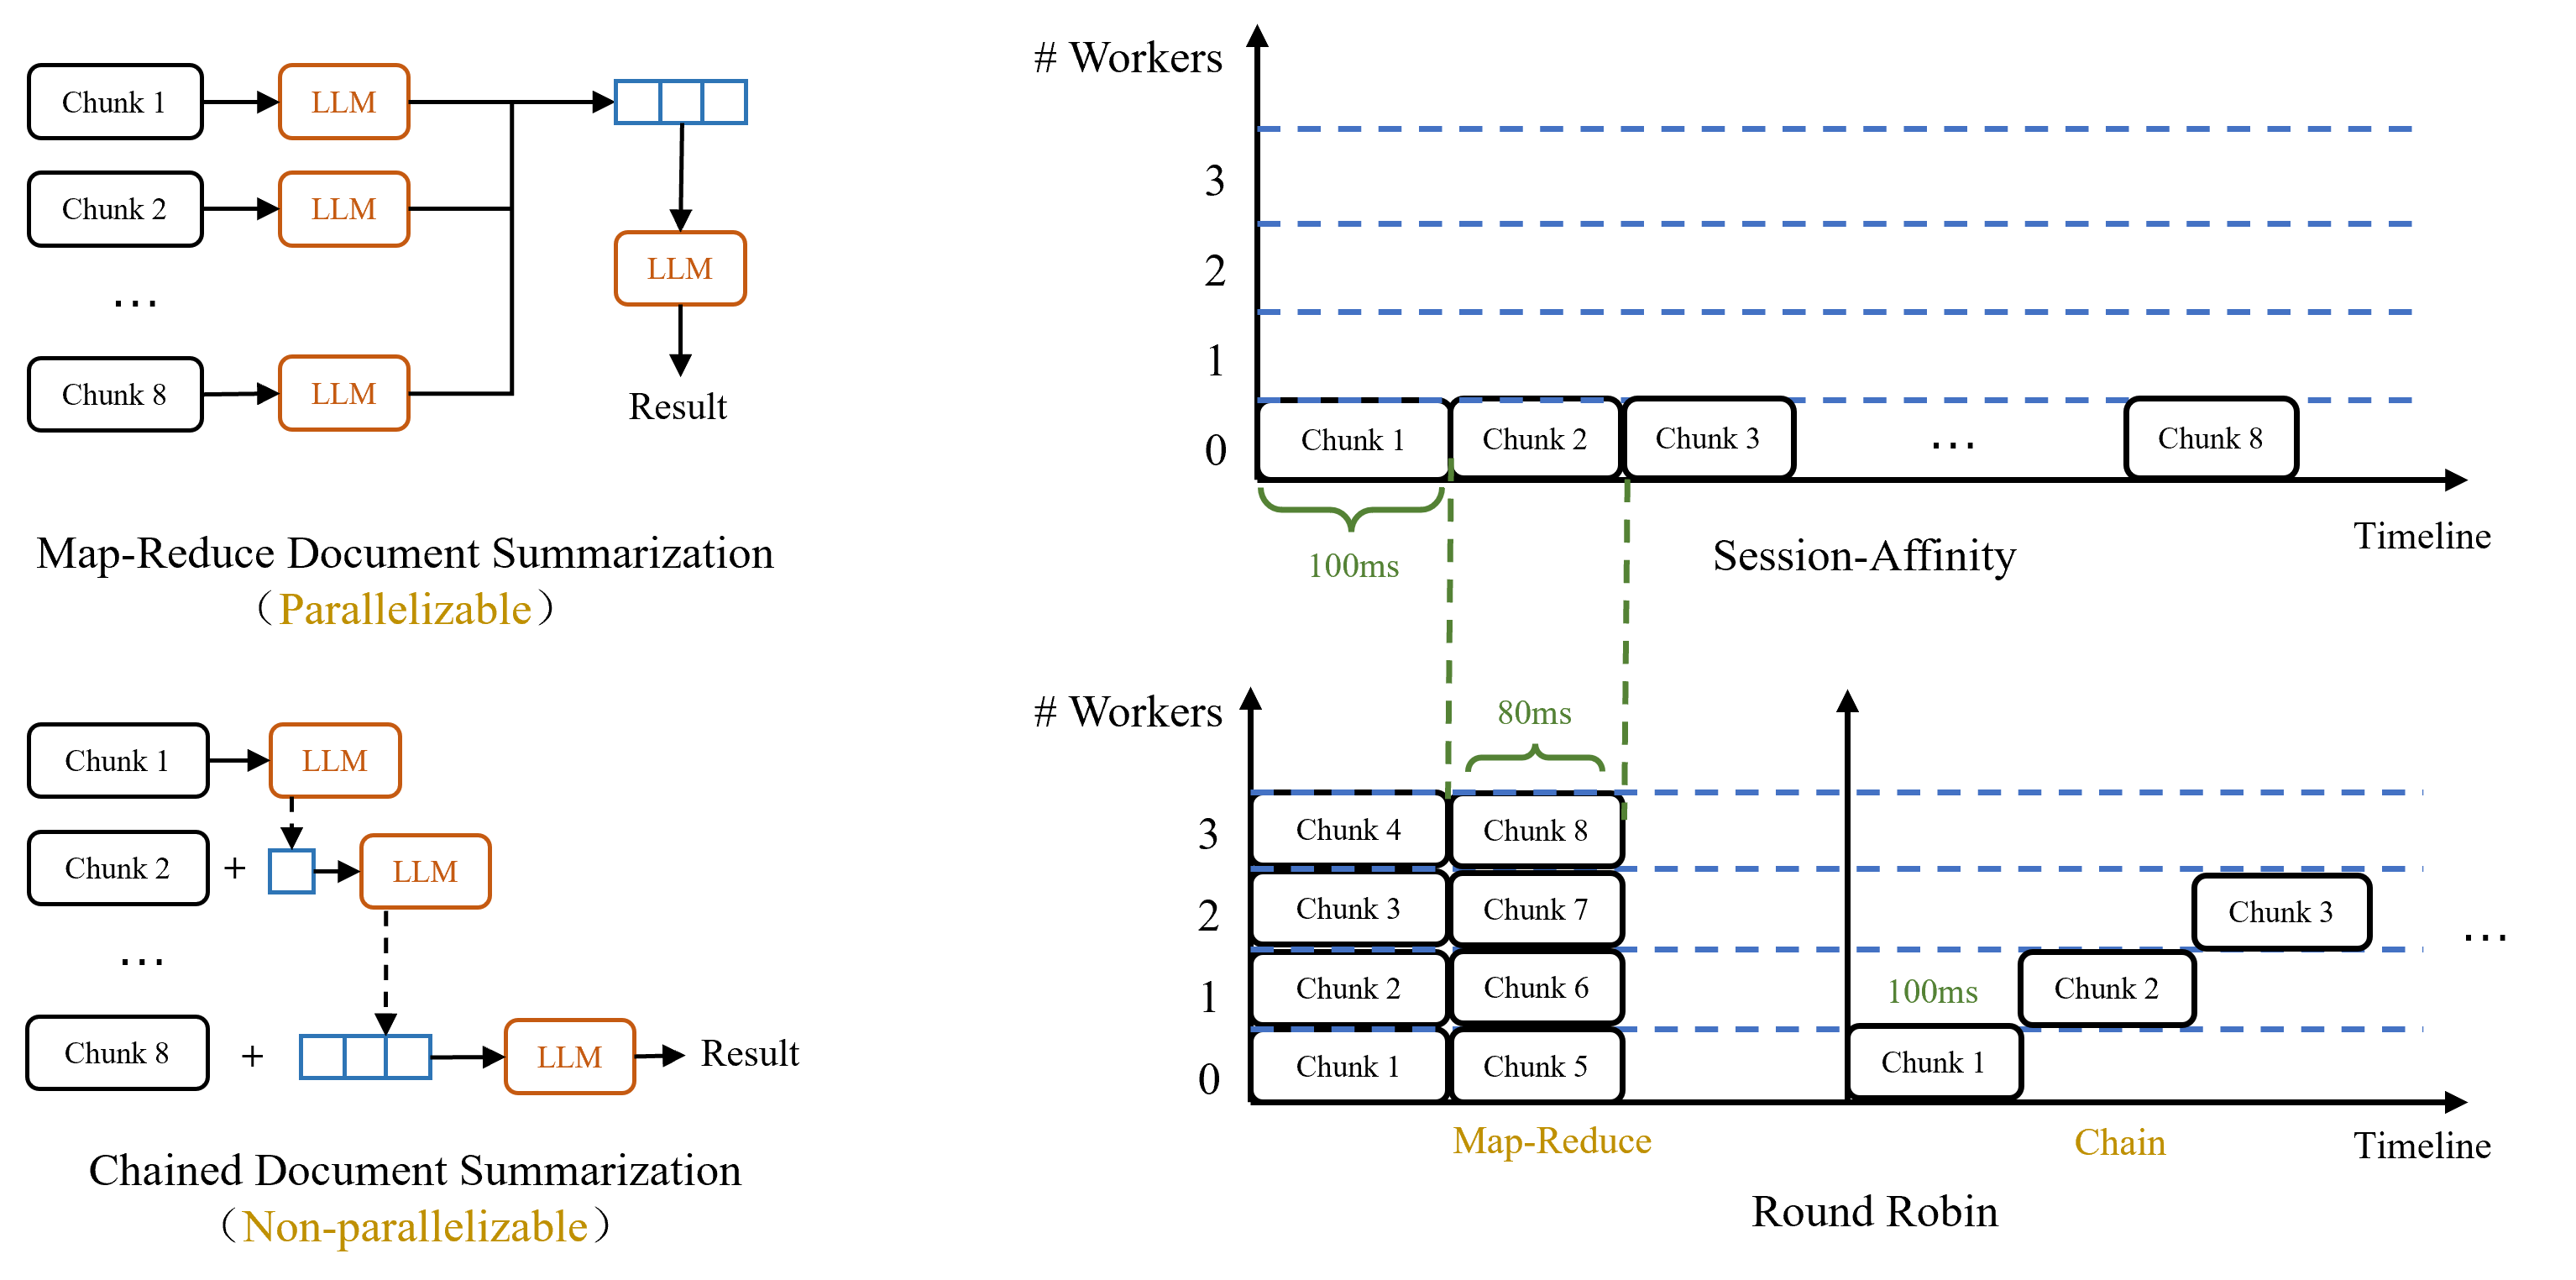
\includegraphics[width=\textwidth]{figures/2.2.png}
    \caption{LLM Agent 输入结构示例}
    \label{fig:llm-agent-input-structure}
\end{figure}

在 LLM Agent 应用场景中，前缀缓存复用的价值尤为突出。
Agent 工作流（Agentic Workflows）通常包含固定的系统提示词、工具调用描述以及多轮对话历史等长前缀，
这些内容在并发请求或单个会话的多轮调用中会大量重复~\cite{lin2024parrot,pan2025kvflow}。
如图~\ref{fig:llm-agent-input-structure} 所示，智能体的输入结构天然呈现出不同粒度的可复用性：
全局静态的系统提示词构成了应用级别的公共前缀，
其键值缓存可在不同用户的并发请求间跨会话复用；动态增长的历史上下文则构成了会话级别的共享前缀，
可在同一用户的多轮交互中被反复命中与追加；而当前用户的输入则是高度个性化且单次有效的，无法进行前缀复用。
通过对这些具有不同生命周期的公共前缀键值缓存进行持久化与跨请求复用，推理引擎能够显著降低海量智能体
请求的预填充计算开销，从而在高并发服务场景下优化请求的首字延迟并提升系统的整体吞吐量。

\subsection{深度强化学习基础}\label{subsec:drl-basics}

深度强化学习（Deep Reinforcement Learning, DRL）~\cite{mnih2013playing,schulman2017proximal}
将深度神经网络的特征表示能力与强化学习的序列决策框架相结合，
能够在高维状态空间中学习复杂的决策策略，
已被广泛应用于游戏博弈~\cite{vinyals2019grandmaster}、机器人控制~\cite{levine2016end}、
资源调度~\cite{peng2021dl2}等领域。
本文第\ref{chap:adasched}章和第\ref{chap:agent-routing}章分别采用了不同的深度强化学习框架
来求解深度学习训练集群调度和LLM Agent推理服务路由问题，本节对相关基础理论进行简要介绍。

\textbf{马尔可夫决策过程。}
强化学习将序列决策问题形式化为马尔可夫决策过程（Markov Decision Process, MDP）~\cite{bellman1957markovian}。
马尔可夫决策过程可定义为五元组$\left(\mathcal{S}, \mathcal{A}, P, R, \gamma\right)$，
其中$\mathcal{S}$为状态空间，$\mathcal{A}$为动作空间，
$P\left(s' \mid s, a\right)$为状态转移概率函数，
$R\left(s, a\right)$为奖励函数，$\gamma \in \left[0, 1\right)$为折扣因子~\cite{kaelbling1996reinforcement}。
在每个时间步$t$，智能体观测当前状态$s_t \in \mathcal{S}$，
根据策略$\pi\left(a \mid s\right)$选择动作$a_t \in \mathcal{A}$，
环境根据转移概率$P$转移到下一状态$s_{t+1}$并返回即时奖励$r_t = R\left(s_t, a_t\right)$。
智能体的优化目标是学习一个最优策略$\pi^*$，使得从任意初始状态出发的期望累积折扣回报最大化：
\begin{equation}\label{eq:rl-objective}
    \pi^* = \arg\max_{\pi} \mathbb{E}_{\pi} \left[ \sum_{t=0}^{\infty} \gamma^t r_t \right].
\end{equation}

\begin{figure}[htbp]
    \centering
    \includegraphics[width=0.6\textwidth]{figures/2.1.png}
    \caption{强化学习示意图}
    \label{fig:rl-loop}
\end{figure}

为了学习并逼近这一最优策略，现有的强化学习算法主要分为两大类：基于值函数的方法与基于策略梯度的方法~\cite{sutton1999reinforcement}。

%\textbf{探索策略与经验回放。}
%强化学习面临探索（exploration）与利用（exploitation）的权衡\cite{}：
%智能体既需要充分探索未知的状态-动作空间以发现更优的策略，
%又需要利用已知的高回报策略来最大化当前收益。
%$\varepsilon$-greedy策略是最常用的探索方法之一，智能体以概率$\varepsilon$随机选择动作进行探索，
%以概率$1 - \varepsilon$选择当前最优动作进行利用。
%在基于策略梯度的方法中，还可以通过在优化目标中引入策略分布的熵正则化项$H(\pi_\theta(\cdot \mid s))$，
%鼓励策略保持适度的随机性，防止过早收敛至局部最优\cite{}。

%经验回放（Experience Replay）\cite{}是稳定深度强化学习训练的关键技术。
%该机制将智能体与环境交互产生的经验样本$(s_t, a_t, r_t, s_{t+1})$存储到一个固定容量的回放缓冲区中，
%训练时从缓冲区中随机采样小批量样本进行参数更新。
%经验回放打破了样本间的时间相关性，使训练数据近似满足独立同分布假设，
%从而提升了神经网络参数更新的稳定性和样本利用效率。
%本文两项工作均采用了经验回放机制来支持离线预训练和在线微调的训练流程。

\textbf{基于策略梯度的方法。}
基于策略梯度的方法~\cite{sutton1999policy}直接用神经网络拟合策略函数$\pi_\theta\left(a \mid s\right)$，
通过梯度上升法优化策略参数$\theta$以最大化期望回报。
REINFORCE算法~\cite{williams1992simple}是最基础的策略梯度方法，其策略梯度估计为：
\begin{equation}\label{eq:reinforce}
    \nabla_\theta J\left(\theta\right) = \mathbb{E}_{\tau \sim \pi_\theta} \left[ \sum_{t=0}^{T} \nabla_\theta \log \pi_\theta\left(a_t \mid s_t\right) \cdot G_t \right],
\end{equation}
其中$G_t = \sum_{k=0}^{\infty} \gamma^k r_{t+k}$为从时间步$t$开始的累积折扣回报。
然而，直接使用蒙特卡洛回报$G_t$作为梯度估计的系数会导致较高的方差，影响训练稳定性。
为此，Actor-Critic架构引入一个价值网络（Critic）$V_\omega\left(s\right)$来估计状态价值函数，
并利用优势函数$A_t = G_t - V_\omega\left(s_t\right)$替代$G_t$进行策略梯度估计，
从而以引入近似偏差为代价显著降低梯度估计的方差。在该架构中，策略网络（Actor）和价值网络
同时进行训练：价值网络通过最小化时序差分误差来逼近真实的状态价值函数，
策略网络则利用价值网络提供的优势估计来更新策略。

\textbf{基于值函数的方法。}
与策略梯度方法不同，基于值函数的方法不直接参数化策略，
而是学习动作价值函数$Q\left(s, a\right)$，并通过贪心策略选择具有最高$Q$值的动作。
深度Q网络（Deep Q-Network, DQN）~\cite{mnih2013playing}利用深度神经网络逼近$Q$函数，
通过最小化时序差分（Temporal Difference, TD）误差来更新网络参数：
\begin{equation}\label{eq:dqn-loss}
    \mathcal{L}\left(\theta\right) = \mathbb{E}_{\left(s_t, a_t, r_t, s_{t+1}\right)} \left[ \left( r_t + \gamma \max_{a'} Q\left(s_{t+1}, a'; \theta^-\right) - Q\left(s_t, a_t; \theta\right) \right)^2 \right],
\end{equation}
其中$\theta^-$为目标网络的参数，通过周期性复制在线网络参数$\theta$来更新，
以提高训练的稳定性。然而，标准深度Q网络存在$Q$值过估计问题，
即最大化操作倾向于选择被高估的动作价值。

Double DQN~\cite{van2016deep}通过解耦动作选择与价值评估来缓解该问题。具体来说，模型中存在两个深度神经网络，
其中在线网络$\theta$用于选择最优动作，而目标网络$\theta^-$用于评估该动作的价值：
\begin{equation}\label{eq2:ddqn-target}
    Y_t^{\text{DDQN}} = r_t + \gamma Q\left(s_{t+1}, \arg\max_{a'} Q\left(s_{t+1}, a'; \theta\right); \theta^-\right).
\end{equation}
该方法在不增加额外计算开销的前提下，有效降低了$Q$值的过估计偏差，提高了策略的质量。

基于策略梯度的方法通过直接优化策略的参数化表示，能够自然地处理多步序列化决策问题，
尤其适用于智能体在单次决策回合中需要执行多步关联动作、
且仅在回合结束时获得延迟奖励信号的场景~\cite{sutton1999policy}；
而基于值函数的方法通过学习状态-动作价值直接评估每个动作的长期收益~\cite{mnih2013playing}，
在每个决策步骤相对独立、反馈信号较为即时的场景中通常具有更高的样本效率。
本文根据两个调度问题的决策结构差异，分别选择了REINFORCE和Double DQN算法，
相关内容将在后续各章的方法设计部分详细介绍。

\section{深度学习训练集群调度研究现状}\label{sec:dl-sched-survey}

%随着深度学习训练任务在共享GPU集群上的大规模部署，如何高效调度这些资源密集型任务已成为系统研究中的核心挑
%战~\cite{ye2024deep}。针对这一挑战，现有研究在分类上主要呈现出两个维度。在资源分配范式上，
%现有调度方法根据任务运行期间资源配置是否可变，可大致分为非弹性调度与弹性调度两类：
%非弹性调度在任务提交时为其分配固定数量的GPU资源，直至任务完成；其中，要求同一任务的所有工作节点
%同时持有GPU资源的调度方式通常称为群组调度（Gang Scheduling）。弹性调度（Elastic Scheduling）
%则允许调度器在任务训练过程中根据集群空闲资源状况动态调整其分配资源量，具有更高的资源利用灵活性。
%%在系统优化目标上，现有工作主要聚焦于任务吞吐量、截止时间满足率以及模型训练性能等核心指标。
%基于上述两个维度，本节从调度方法出发，在各小节内部按非弹性/弹性调度的顺序，梳理深度学习集群调度领域的研究进展。

随着深度学习训练任务在共享GPU集群上的大规模部署，如何高效调度这些资源密集型任务已成为系统研究中的核心挑战~\cite{ye2024deep}。
针对这一挑战，现有的调度策略在分类上主要可划分为两个维度。首先，在算法类型上，现有的调度工作主要分为三类：基于启发式算法的调度、
基于数学求解器的调度以及基于强化学习的调度。
其次，在资源分配范式上，上述各类调度方法的发展均呈现出从传统的非弹性调度向更灵活的弹性调度（Elastic Scheduling）演进的趋势：
非弹性调度在任务提交时为其分配固定数量的GPU资源直至任务完成（如，群组调度）；
而弹性调度则允许调度器在训练过程中根据集群资源状况动态伸缩任务的资源分配量。
基于上述两个维度，本节将以调度算法的类型为主要脉络展开分类讨论，并在各小节内部按照从非弹性调度到弹性调度的演进顺序，
系统梳理深度学习集群调度领域的研究进展。

\begin{table}[htbp]
    \centering
    \small % 适当缩小字号以适应页面
    \setlength{\tabcolsep}{4pt} % 稍微收紧列间距
    \begin{threeparttable}
      \caption{深度学习训练集群调度代表工作汇总}
      \label{tab:dl-sched-survey}
      % 使用 tabularx 自动调整列宽，X 代表自动扩展列
      \begin{tabularx}{\textwidth}{c c c c}
        \toprule
        调度策略   &文献        & 弹性调度                                    & 优化目标                                                   \\
        \midrule
        \multirow{7}{*}{启发式算法} & Tiresias~\cite{gu2019tiresias}，HiveD~\cite{zhao2020hived}       & \ding{55}          & JCT     \\
                                   & Optimus~\cite{peng2018optimus}  & \ding{51}                   & JCT  \\
                                   & Pollux~\cite{qiao2021pollux}，Sia~\cite{jayaram2023sia}  & \ding{51}                   & JCT，公平性  \\
                                   & ElasticFlow~\cite{gu2023elasticflow}  & \ding{51}        & SLO  \\
                                   & SLAQ~\cite{zhang2017slaq}  & \ding{51}        & JCT，模型性能  \\
                                   & HyperDrive~\cite{rasley2017hyperdrive}  & \ding{55}        & JCT，模型性能  \\
                                   & Rubberband~\cite{misra2021rubberband}  & \ding{51}        & 资源利用率，模型性能  \\
        \midrule
        \multirow{2}{*}{数学求解器} & Chronus~\cite{gao2021chronus}，Unisched~\cite{gao2024unisched}  & \ding{55}        & JCT，SLO  \\
                                   & Gavel~\cite{narayanan2020heterogeneity}  & \ding{55}        & JCT，公平性  \\
        \midrule
        \multirow{3}{*}{强化学习算法} & DeepRM~\cite{mao2016resource}  & \ding{55}        & JCT  \\
                                   & MLFS~\cite{wang2020job}  & \ding{55}        & JCT，模型性能  \\
                                   & DL2~\cite{peng2021dl2}  & \ding{51}        & JCT  \\
        \bottomrule
      \end{tabularx}
    \end{threeparttable}
  \end{table}


%\subsection{优化任务完成时间的调度方法}
\subsection{基于启发式算法的调度方法}\label{subsec:heuristic}

在多租户GPU集群中，调度器通常以优化平均任务完成时间（Job Completion Time, JCT）或集群整体吞吐量为主要
目标。从非弹性调度的角度，针对该场景下深度学习训练时间难以预知导致严重排队延迟的问题，
Tiresias~\cite{gu2019tiresias} 提出了一种基于“二维已获得服务”（2DAS）的启发式调度算法。
该方法根据任务已消耗的 GPU 时长动态调整优先级，并在分布式作业调度时，智能判定何时放宽传统的严格拓扑放置约束。
这种策略在无需额外用户输入的情况下显著降低了高负载集群下的排队延迟，从而最小化系统平均任务完成时间。

HiveD~\cite{zhao2020hived}观察到在多租户GPU集群中仅仅基于数量配额（Quota）的调度会导致严重的不公平性，
进而影响不同用户所提交任务的完成时间与系统吞吐量。
为此，HiveD 提出了一种保障“共享安全”的资源预留框架。该框架创造性地引入
了多级单元结构来刻画物理集群中不同级别的 GPU 亲和性，并结合伙伴单元分配算法，为每个租户构建出虚拟
的私有集群抽象。基于这一抽象，系统不仅允许各类现有调度策略透明接入，更在资源的全局共享与租户隔离
保护之间，实现了高效且均衡的分配。然而，上述两种算法均仅支持静态的群组调度机制，
无法动态调整任务的GPU分配数量，限制了集群资源的利用率。

%针对静态独占分配导致资源利用率低下的问题，Gandiva~\cite{xiao2018gandiva} 结合深度学习任务在微批次（Mini-batch）
%迭代内的高度可预测性，提出了一种基于性能内省（Introspection）的细粒度动态时空共享机制。该框架通过透明的任务迁移与时间分片，
%实现了多作业对 GPU 的高效复用，在满足超参数探索低延迟需求的同时显著提升了系统的整体并发度。

随着弹性调度技术的发展，系统开始支持在训练过程中动态调整计算资源。
针对静态分配无法最小化作业完工时间的问题，Optimus~\cite{peng2018optimus} 提出了一种基于在线性能建模的启发式弹性调度算法。
该方法通过实时拟合收敛曲线建立资源与训练速度的映射，并利用基于边际收益的贪心策略，动态调整各任务的资源配额与放置方式。
此举在保障模型收敛的同时，显著缩短了任务完成时间并提升了集群吞吐量。
然而，Optimus仅适合基于参数服务器（Parameter Server）架构的分布式深度学习训练集群，无法直接应用于主流的All-Reduce分布式训练范式。

针对底层资源分配与上层超参数配置脱节导致训练效率低下的问题，Pollux~\cite{qiao2021pollux}
引入了兼顾系统硬件吞吐与模型统计效率的“有效吞吐量”（Goodput）指标，将计算资源的弹性伸缩与批次大小、学习率的动态调整联合建模为协同优化问题。
该方法通过基于种群的进化算法持续搜索最优配置，在保障多租户公平性的同时，显著提升了集群整体与单任务的执行效率。然而，这种基于进化算法的搜索策略
在面对大规模集群时存在严重的计算瓶颈，无法满足在线动态调度的实时性要求。

此外，Optimus和Pollux均仅面向同构集群。
为应对现代数据中心广泛存在的硬件异构性挑战，Sia~\cite{jayaram2023sia}在Pollux的基础上提出了一种面向异构计算集群且
支持深度学习自适应弹性架构的高效调度方法。
该方法构建了异构硬件的吞吐量分配模型，并动态将任务精准映射至当前性能最优的 GPU 节点组合。
此举在应对剧烈波动的真实异构负载时，显著提升了集群的整体吞吐性能与资源利用率。

在实际的生产环境中，许多深度学习训练作业受到严格的截止期限或服务等级目标（Service Level Objective，SLO）的约束。
因此，许多工作将调度器的核心优化目标设置为最大化在截止期限前顺利完成的作业比例。
在非弹性调度场景下，最早截止期限优先（Earliest Deadline First, EDF）作为经典的实时调度算法，
通过将计算资源倾斜分配给截止期限最紧迫的任务来保障服务的及时性。

ElasticFlow~\cite{gu2023elasticflow}则提出了一种面向分布式深度学习的
弹性无服务器（Serverless）训练平台。
针对训练吞吐量随 GPU 规模呈非线性扩展以及分布式节点放置所带来的系统性挑战，
该工作引入了“最小满意份额”（Minimum Satisfactory Share）的评估指标，精确量化了满足作业截止期限所需的
最小资源量。基于该动态份额，ElasticFlow 实施了严格的准入控制，并结合基于边际收益递减的贪心算法与
伙伴分配策略，不仅显著降低了用户提交任务时的配置复杂度，还大幅提升了集群整体的截止期限满足率。

部分研究还关注到模型性能对调度决策的直接影响，旨在将有限的计算资源分配给性能提升潜力更大的任务。
SLAQ~\cite{zhang2017slaq}通过在线监测训练过程中损失函数的下降速率来评估任务进度，
并将资源优先分配给边际收益更高的任务，从而加速整体模型群的收敛。然而，SLAQ 的资源分配模型仅针对 CPU 集群
设计，未能涵盖现代深度学习高度依赖的 GPU 调度场景。

然而，在当前的深度学习集群调度研究中，直接将模型最终性能作为资源分配依据的工作相对较少，
且这类性能感知的调度策略主要集中在超参数调优（Hyperparameter Optimization, HPO）领域。
在 HPO 场景中，由于超参数搜索通常需要耗费大量的训练时间和计算资源，HyperDrive~\cite{rasley2017hyperdrive}
提出了一种兼顾训练效率与模型质量的超参数调优平台框架。
该框架首先结合概率模型与提前终止技术，快速评估并辨别各类超参数配置的优劣；在此基础上，调度器动态调整不同试验的
资源分配比重，将计算资源向潜力更高的配置倾斜，最终实现整体调优耗时与资源开销的平衡。

针对云环境下 HPO 集群规模固定导致资源严重闲置的问题，Rubberband~\cite{misra2021rubberband} 深入挖掘了搜索阶段可用并行度的动态变化特征。
该框架结合底层计算性能分析（Profiling）与云服务计费模型，将弹性资源调度建模为带有时间约束的成本最小化问题。
系统通过在运行时动态生成最优的集群伸缩策略，优先为高潜力的搜索分支倾斜算力，在严格保障截止期限的同时显著降低了云实例的租赁总成本。

然而，现有截止期限感知的调度方法主要依赖用户给定的不准确的迭代次数估计，
缺乏对最终模型性能指标的直接优化；而现有的性能感知调度方法往往缺乏截止期限支持，
或仅局限于超参数调优相关的特定场景。如何在满足截止期限的前提下最大化通用训练任务的模型收敛收益，仍是当前集群调度领域尚未解决的问题。
%本文第\ref{chap:adasched}章将针对这一空白，
%提出将模型验证目标性能作为完成条件的调度机制，并同时支持基于截止期限约束的弹性资源分配。

%\subsection{优化截止时间满足率的调度方法}
\subsection{基于数学求解器的调度方法}\label{subsec:solver}
尽管前文所述的各类启发式算法能够在可接受的时间开销内快速生成调度方案，但这类方法本质上依赖于经验规则或概率搜索，
缺乏对全局最优性的严谨数学保证。在面临复杂的集群环境与多维度的严格约束（如任务依赖、截止期限等）时，
启发式算法极易陷入局部最优，最终往往只能提供次优的调度决策，造成潜在的资源浪费与性能折损。
为了克服这一固有局限，部分研究工作放弃了启发式的局部探索，转而将系统调度过程严格形式化为数学规划模型，
并依赖成熟的数学求解器进行全局最优化。

针对混合工作负载中如何兼顾 SLO 作业的严格截止期限与尽力而为（Best-effort）作业的执行效率问题，
Chronus~\cite{gao2021chronus}利用深度学习训练的高度可预测性，将基于租约的抢占式调度严格建模为混合整数线性规划（MILP）问题。
系统通过求解器计算出结合准入控制的时间切片分配方案，在提供严格 SLO 期限保障的同时最大化了 Best-effort 作业的吞吐。
然而，Chronus 依然局限于静态的群组调度范式，这种缺乏弹性的机制限制了系统容纳更多任务的潜力，
导致其无法实现截止时间满足率的全局最大化。

UniSched~\cite{gao2024unisched}针对 Chronus 中任务选择与资源分配相分离导致的次优解问题，
将任务分析、资源分配与底层拓扑资源映射统一建模为一个全局 MILP 优化问题。通过求解器对时间与空间维度进行联合优化，
UniSched 不仅进一步显著降低了 SLO 违约率，还将 Best-effort 作业的延迟大幅缩短。
然而，受限于巨大解空间带来的高昂搜索开销，该算法难以支持训练中途动态调整 GPU 数量的弹性伸缩机制。

针对现有深度学习集群调度器忽视异构资源性能差异的问题，Gavel~\cite{narayanan2020heterogeneity}将各类宏观的集群调度策略
（如公平性、最小化 JCT 等）统一转化为基于“有效吞吐量”的数学最优化问题。
系统通过调用现成的求解器计算出最优的时分复用资源分配矩阵，随后利用一种基于轮转的调度机制来严格执行该分配。
相比于不感知异构的调度策略，Gavel虽大幅降低了集群平均任务完成时间和整体完工时间，但其同样难以适配弹性调度场景。

然而，此类方法在实际部署中面临严峻的可扩展性与时效性瓶颈。
集群多维资源调度本质上属于高度复杂的 NP-Hard 问题，导致数学求解器的计算开销随集群规模与并发任务量的增加呈指数级增长，
决策延迟高达数百乃至数千秒。面对真实数据中心秒级甚至毫秒级的瞬时响应要求，
这种难以承受的算法开销使其无法适应现代集群对高吞吐与低延迟实时调度的严苛需求。

%\subsection{优化模型性能的调度方法}
\subsection{基于强化学习的调度方法}
如前文所述，深度学习训练集群调度可归结为高度动态环境下的在线序列决策问题。
面对该问题，传统的启发式方法缺乏动态适应性，难以保证所得解的质量，
而数学规划方法在面对大规模问题时存在严重的计算瓶颈~\cite{gao2021chronus,qiao2021pollux}。
深度强化学习因其能够在高维状态空间中通过与环境交互自动学习高质量的调度策略，
逐渐成为解决此类复杂系统调度问题的有力工具。

DeepRM~\cite{mao2016resource}是最早将深度强化学习应用于资源管理的工作之一，
其将多资源调度问题建模为马尔可夫决策过程，并使用策略梯度方法训练调度策略，
证明了强化学习方法在资源调度场景中能够学习到优于经典启发式算法的策略。
然而，DeepRM的状态和动作空间设计相对简单，且仅支持传统机器学习任务，难以直接扩展到大规模GPU集群场景。

针对深度学习训练的多目标调度问题，MLFS~\cite{wang2020job} 构建了一种结合离线启发式预训练与在线强化学习微调的调度系统。
该系统综合考量任务的时空与计算特征，并引入基于损失曲线的动态终止机制，
实现了任务完成时间、精度和截止期限满足率的联合优化。
然而，MLFS 仍局限于静态的群组调度范式，无法在运行时动态调整任务的 GPU 资源；
此外，其决策过程缺乏对底层网络拓扑的感知，极易在分布式训练中引发通信瓶颈。

针对参数服务器架构下分布式深度学习的弹性资源分配问题，
DL2~\cite{peng2021dl2} 同样提出了一种混合强化学习调度框架。
为缓解强化学习的冷启动问题，DL2 首先利用离线监督学习拟合现有启发式调度器（如 DRF）的历史决策轨迹来初始化策略网络。
随后，结合 REINFORCE 算法与动作掩码机制，
在真实环境中进行在线策略微调与高效探索。
实验表明，相较于 DRF 和 Optimus，DL2 能显著降低平均任务完成时间。
然而，其调度策略仅以最小化 JCT 为单一优化目标，缺乏对截止期限约束与模型训练性能等复杂系统需求的综合考量。

%尽管上述工作为强化学习在集群调度中的应用奠定了基础，但仍存在一定的局限性。DeepRM 和 DL2 主要以任务完成时间等系统级指标为优化目标，
%未能将模型内在的训练性能纳入决策过程；MLFS 虽然引入了模型精度指标，但其采用静态调度机制，无法动态支持资源的弹性分配。
%总体而言，现有的强化学习调度方法尚未能在统一的框架下，实现性能感知、截止期限保障与弹性资源调度的协同优化。

尽管上述工作验证了强化学习在集群调度中的潜力，但在现代 AI 负载的多维约束下，
现有方法存在明显的优化维度割裂：侧重资源弹性与系统效率的方案未能兼顾模型训练性能与截止期限；
而引入多目标优化的系统则多局限于静态调度，缺乏动态资源伸缩能力。
总体而言，现有研究尚未能在统一框架下实现性能感知、期限保障与弹性调度的协同优化。

\section{大语言模型推理集群调度研究现状}\label{sec:llm-sched-survey}

随着大语言模型在众多智能应用场景中的广泛部署，
LLM推理集群的调度优化日益受到学术界和工业界的关注~\cite{gexuran2025,zhou2024surveyefficientinferencelarge,yi2025edgemoeempoweringsparselarge}。
当前主流的LLM推理集群往往采用全局-本地两级调度架构，如图~\ref{fig:agent-system-arch} 所示。
系统由一个全局调度器（Global Scheduler）和多个本地调度器（Local Scheduler）组成，
全局调度器负责接收用户提交的推理请求并将其分发至本地推理引擎实例；
而本地调度器则部署在各个推理引擎实例上，负责管理单实例范围内的请求排队、批处理与推理执行流程。
与传统的独立服务请求相比，基于大语言模型的智能体工作流在执行阶段展现出更为复杂的动态特性：
不仅请求间存在严格的拓扑依赖，而且智能体功能角色的多样性导致了显著的推理延迟差异。
这些特性对系统的全局精细化调度能力提出了更高要求。
本节从 LLM 推理系统调度方法和 LLM Agent 推理系统调度方法两个维度，
系统梳理当前的研究现状。

\begin{figure}[htbp]
    \centering
    \includegraphics[width=0.6\textwidth]{figures/4.1.png}
    \caption{LLM推理集群的分层调度架构}
    \label{fig:agent-system-arch}
\end{figure}


\begin{table}[htbp]
    \centering
    \small % 适当缩小字号以适应页面
    \setlength{\tabcolsep}{4pt} % 稍微收紧列间距
    \begin{threeparttable}
      \caption{大语言模型推理集群调度代表工作汇总}
      \label{tab:llm-sched-survey}
      % 将第三列（文献）设为 X 列，使其自动换行并撑满页面宽度
      \begin{tabularx}{\textwidth}{c c X c}
        \toprule
        调度对象 & 优化层级 & 文献 & 优化目标 \\
        \midrule
        
        % 第一大块：LLM 请求 (跨6行)
        \multirow{6}{*}{LLM 请求} & \multirow{3}{*}{引擎层} & vLLM~\cite{kwon2023efficient} & 显存利用率 \\
        % 下面两行因为前两列都被 multirow 占了，所以需要两个 & 占位
                                  &                         & Sarathi-Serve~\cite{agrawal2024taming} & TTFT，TPOT，吞吐量 \\
                                  &                         & SGLang~\cite{zheng2024sglang}          & TTFT \\
        \cmidrule{2-4} % 关键：只在第 2 到第 4 列画线，不穿透第一列
        
                                  & \multirow{3}{*}{集群层} & DynamoLLM~\cite{stojkovic2025dynamollm}& SLO \\
                                  &                         & AIBrix~\cite{team2025aibrix}           & 请求时延，SLO，吞吐量 \\
                                  &                         & TORTA~\cite{du2025temporal}            & 请求时延 \\
        \midrule % 调度对象切换，画一条完整的横线
        
        % 第二大块：LLM Agent 工作流 (跨3行)
        \multirow{3}{*}{LLM Agent工作流} & \multirow{3}{*}{集群层} & Parrot~\cite{lin2024parrot}, Ayo~\cite{tan2025towards} & E2E延迟，吞吐量 \\
                                         &                        & Autellix~\cite{luo2025autellix}，Kairos~\cite{chen2025kairos}，KVFlow~\cite{pan2025kvflow} & E2E延迟 \\
                                         &                        & HexGen-Flow~\cite{peng2025hexgen} & SLO \\
        \bottomrule
      \end{tabularx}
    \end{threeparttable}
  \end{table}

\subsection{LLM 推理系统调度研究现状}\label{subsec:llm-routing}

为了提升分布式集群下的推理服务吞吐量并降低推理延迟，
现有工作针对LLM推理过程中的显存管理、请求批处理、前缀缓存机制和集群资源分配等关键问题，
提出了一系列全局调度系统架构及优化策略。

在显存管理与连续批处理方面，vLLM系统借鉴操作系统中的虚拟内存分页技术来管理庞大的 KV Cache，
消除了请求序列内部和请求之间的显存碎片。
在集群部署层面，vLLM提供了多实例管理接口，支持基于轮询等经典负载均衡策略进行全局请求路由。
Sarathi-Serve~\cite{agrawal2024taming} 提出了 Chunked-Prefills 机制，
将长上下文的预填充阶段拆解为多个较小的计算块。通过将新请求的预填充块与现有请求的解码步骤进行细粒度交错执行，
该系统有效消除了批处理过程中的流水线气泡，显著提升了高并发场景下的调度性能。

针对高并发大语言模型推理中因共享上下文前缀而引发的计算与显存冗余问题，
SGLang~\cite{zheng2024sglang} 构建了一种基于基数树的细粒度缓存管理框架。
其底层的 RadixAttention 机制通过高效追踪全局历史序列状态，实现了跨请求键值缓存的无缝共享与复用。
依托该底层抽象，系统进一步设计了缓存感知的全局路由算法。
该算法通过精确匹配请求前缀与各实例的缓存驻留状态实施亲和性分发，从而显著减少了冗余的预填充计算开销。

在更宏观的云原生集群与资源管理层面，
计算资源异构性和动态工作负载使得集群全局性能优化变得尤为复杂。
作为首个 LLM 推理集群性能优化框架，DynamoLLM~\cite{stojkovic2025dynamollm} 通过量化分析推理性能的异构性，
实现了受 SLO 延迟约束的集群资源动态重配置。具体而言，该框架能够依据实时请求负载和模型属性，
自适应地调节服务实例数、模型并行策略乃至底层 GPU 的运行频率。
AIBrix~\cite{team2025aibrix} 构建了一套云原生的大语言模型推理基础设施。在底层机制上，该系统支持跨节点的键值缓存
共享与 LoRA 适配器的动态加载；在全局路由层面，AIBrix 引入了融合前缀匹配与负载感知的复合调度策略。通过在缓存
命中收益与集群算力均衡之间进行动态折中，该系统有效保障了大规模 LLM 服务的高效运行。

相较于在深度学习训练调度领域的日趋成熟，强化学习在 LLM 推理调度中的应用探索仍处于起步阶段。
TORTA~\cite{du2025temporal}针对分布式 LLM 推理基础设施，基于强化学习构建了一个跨区域流量分配器，
通过动态调整时间窗口内的请求路由比例，有效缓解了局部集群的资源瓶颈。
%RLoT~\cite{hao2025rl}则面向结构复杂的 LLM 智能体应用，训练了一个轻量级强化学习规划器，
%能够为异构任务动态生成最优的推理计算图，从而在严控开销的前提下显著提升推理质量。

然而，上述方法大多局限于单一的 LLM 推理服务，缺乏对任务间复杂依赖关系的建模能力，
因此难以直接推广到多智能体协同的复杂工作流调度场景。

\subsection{LLM Agent 推理系统调度研究现状}\label{subsec:agent-sched}

相较于上述面向独立、离散请求的标准 LLM 推理服务，智能体工作流以大语言模型为推理核心，
通过多轮工具调用与环境交互来完成复杂任务。这种执行模式使得底层的推理请求不再独立，
而是组织成具有严格拓扑依赖关系的复杂工作流。
针对智能体应用的请求依赖结构和推理异构性，
学术界提出了一系列专门针对多步协作型任务和工作流特性而优化设计的调度系统。

作为首个深入探讨智能体工作流调度的研究工作，Parrot~\cite{lin2024parrot} 针对传统推理引擎将请求孤立处理的局限性，
提出了一种名为语义变量的编程抽象。该抽象通过对智能体工作流中复杂的输入输出依赖与数据流进行显式建模，
将原本离散的推理请求重构为结构化的逻辑计算图。
通过向底层推理服务传递此类应用层语义，Parrot 借鉴编译器分析技术在运行时动态提取拓扑依赖。
在全局调度层面，该系统引入了基于会话亲和性（Session Affinity）
的分发策略，将共享相同上下文前缀的请求定向至特定节点，从而最大化了键值缓存的跨请求复用率。

针对现有 LLM 框架仅提供模块级粗粒度接口的局限性，Ayo~\cite{tan2025towards} 提出了一种细粒度的任务原语编排框架。
该系统将复杂的应用工作流解耦为原语级的数据流图，消除了传统执行框架中粗粒度模块对底层执行逻辑的黑盒封装。
在调度层面，Ayo 不仅设计了感知拓扑深度的批处理策略，还创新性地在分布式集群中实现了 LLM 计算阶段（如预填充与解码）
与非 LLM 模块（如向量检索与重排）的流水线并行。这种全链路的协同机制，显著降低了典型 LLM 应用的端到端延迟。

与Parrot类似，Autellix~\cite{luo2025autellix}将完整的智能体工作流而非单次LLM请求作为独立调度单元。
借鉴操作系统的进程调度思想，该系统提出了 PLAS 及其并行扩展 ATLAS 算法。
其底层依托多级反馈队列构建抢占式调度机制，以程序已累积的执行时间（或关键路径上的累积时间）为核心指标，
对全局请求进行动态映射与重排。
通过这种调度策略，Autellix 有效缓解了请求级与程序级的队头阻塞问题。

针对多智能体工作流中由于异构节点角色带来的显著跨节点延迟差异问题，
Kairos~\cite{chen2025kairos} 提出了一种基于工作流感知的优先级调度与显存分发框架。
在调度决策层面，该系统通过解析智能体任务的有向无环图（DAG）结构并收集历史延迟分布，
采用基于预期剩余执行时间的优先级排队策略与动态装箱机制实施资源分配，
从而有效降低了高吞吐场景下的显存溢出概率。

针对多租户异构 GPU 集群下多阶段 Text-to-SQL 工作流的延迟保障问题，HexGen-Flow~\cite{peng2025hexgen} 
提出了一种结合负载感知与 SLO 感知的两级调度架构。在全局调度层面，该系统综合实例性能模型与实时排队深度实施异构请求分发；
同时，通过将端到端 SLO 按计算量比例细化为请求级时间预算，并引入基于预算余量的紧迫度指标，
实现了对关键请求的抢占式优先调度并有效提升了异构环境下的任务达标率。
然而，该框架深度绑定于特定的 Text-to-SQL 场景，其依赖静态预估的预算拆解机制难以向拓扑更复杂、
执行更具动态性的通用 Agent 工作流扩展。

针对多智能体工作流中频繁的上下文缓存换入换出引发的调度延迟瓶颈，KVFlow~\cite{pan2025kvflow} 
提出了一种工作流感知的精细化缓存调度策略。在方法设计上，该系统通过构建智能体执行图显式建模任务拓扑，
并基于预估的执行距离为缓存节点分配优先级；
进而结合后台异步预取与基于未来重用概率的淘汰机制，有效克服了传统 LRU 算法的盲目性。
这些机制显著提升了缓存命中率并降低了端到端推理延迟。

%针对直接影响调度延迟的智能体前缀缓存管理问题，KVFlow~\cite{pan2025kvflow}提出了一种工作流感知的精细化缓存策略。
%该系统构建智能体执行图以显式建模任务间的拓扑依赖，并基于预估的执行时间距离为各节点分配优先级。
%在缓存淘汰层面，KVFlow 摒弃了传统 LRU 算法的盲目性，优先驱逐未来重用概率较低的缓存节点；
%在预取调度层面，该系统利用工作流先验信息，在后台异步地将后续所需的缓存从 CPU 预加载至 GPU。

尽管上述方法在特定场景下取得了进展，但在全局请求路由层面，现有方案仍高度依赖基于规则的静态启发式策略，
鲜有工作将强化学习应用于智能体工作流的全局分发中。
由于缺乏对系统底层动态状态（如实例实时负载分布、KV Cache 驻留情况等）的深度感知，
现有的静态路由机制往往陷入次优的二元化调度困境：
要么过度追求缓存亲和性导致热点实例过载，要么为了强制负载均衡而将强相关的时序请求分散，引发不必要的键值重算开销。

针对上述问题，强化学习提供了一种打破静态规则瓶颈的解决方案。
引入强化学习的必要性在于，智能体工作流中多步请求间存在着深度的时序依赖与上下文耦合，
这要求调度器不能仅局限于单次请求的贪心分配，而必须优化系统的长期累积回报。
通过将 LLM 推理集群建模为交互环境，强化学习智能体能够综合观测包含队列深度、显存状态及工作流依赖在内的高维状态空间，
自主学习并逼近最优的路由策略。这种自适应的全局调度机制，能够有效在最小化端到端延迟与最大化全局吞吐量之间实现动态权衡，
从而解决传统方法难以应对的在线决策问题。


%\subsection{基于强化学习的LLM推理集群调度研究现状}\label{subsec:rl-llm-sched}

%相较于在深度学习训练调度领域的日趋成熟，强化学习在 LLM 推理服务调度中的应用探索仍处于起步阶段。
%TORTA~\cite{du2025temporal}针对分布式 LLM 推理基础设施，基于强化学习构建了一个跨区域流量分配器，
%通过动态调整时间窗口内的请求路由比例，有效缓解了局部集群的资源瓶颈。
%RLoT~\cite{hao2025rl}则面向结构复杂的 LLM 智能体应用，训练了一个轻量级规划器，能够为异构任务动态生成最优的推理计算图，
%从而在严控开销的前提下显著提升推理质量。

%然而，聚焦于请求路由层面，当前主流方案仍高度依赖基于规则或加权启发式的静态策略，并未考虑引入强化学习
%进行求解。尤其是在处理 LLM 智能体工作流时，由于任务往往伴随复杂的上下文依赖与异构计算特征，
%现有的静态路由机制难以深度感知系统底层的动态运行状态（如实例负载分布、KV Cache 命中率以及工作流的全局执行进度），
%从而无法做出自适应的全局调度决策。


%\section{基于强化学习的集群调度研究现状}\label{sec:rl-sched-survey}

%如第\ref{sec:dl-sched-survey}节和第\ref{sec:llm-sched-survey}节所述，
%深度学习集群调度与 LLM 推理服务调度的核心，均可归结为高度动态环境下的在线序列决策问题。
%传统的启发式方法（如EDF、轮询）缺乏动态适应性，难以保证所得解的质量，
%而数学规划方法（如Chronus的MILP求解）在面对大规模问题时存在严重的计算瓶颈~\cite{gao2021chronus,qiao2021pollux}。
%深度强化学习因其能够在高维状态空间中通过与环境交互自动学习高质量的调度策略，
%逐渐成为解决此类复杂系统调度问题的有力工具。

%\subsection{强化学习在深度学习训练系统调度中的应用}\label{subsec:rl-dl-sched}
%\subsection{基于强化学习的深度学习训练集群调度研究现状}\label{subsec:rl-dl-sched}

%DeepRM~\cite{mao2016resource}是最早将深度强化学习应用于资源管理的工作之一，
%其将多资源调度问题建模为马尔可夫决策过程，并使用策略梯度方法训练调度策略，
%证明了强化学习方法在资源调度场景中能够学习到优于经典启发式算法的策略。
%然而，DeepRM的状态和动作空间设计相对简单，且仅支持传统机器学习任务，难以直接扩展到大规模GPU集群场景。

%MLFS~\cite{wang2020job}结合任务的时空特征（如早期迭代更高的精度收益、模型分区大小）与传统计算特征（如截止期限）设计优先级函数。
%系统先通过启发式调度策略收集数据来预训练强化学习模型，待收敛后切换为强化学习进行在线决策，
%以联合优化任务完成时间、精度和截止期限满足率等指标。
%此外，MLFS还提出了最优迭代停止方法，根据损失曲线自动判断训练终止时机，
%避免无效迭代对资源的浪费。
%然而，该系统在优化带宽成本时未考虑底层的网络拓扑结构对分布式训练任务的影响，
%且仅支持静态的群组调度机制，无法动态调整任务的GPU分配数量。

%针对基于参数服务器（Parameter Server）架构的分布式深度学习训练集群的弹性资源分配问题，
%DL2~\cite{peng2021dl2} 提出了一种结合离线监督预训练与在线强化学习的混合训练范式。
%为缓解强化学习的冷启动问题，DL2 首先利用离线监督学习，通过拟合现有启发式调度器（如 DRF）的历史决策轨迹来初始化策略网络，
%从而避免探索初期的次优决策。随后，该系统在真实集群中引入 REINFORCE 算法，
%根据实际环境的交互反馈对调度策略进行在线微调与持续优化。
%此外，DL2还设计了任务感知的探索机制，
%在采样阶段直接屏蔽明显非法的资源分配动作（如分配多个工作节点却无参数服务器），
%从而提高动作空间探索效率。
%实验表明DL2在平均任务完成时间上显著优于DRF和Optimus等对比方法。
%然而，DL2以最小化平均任务完成时间为唯一优化目标，
%并未考虑截止期限约束和模型训练性能等因素。

%尽管上述工作为强化学习在集群调度中的应用奠定了基础，但仍存在一定的局限性。DeepRM 和 DL2 主要以任务完成时间等系统级指标为优化目标，
%未能将模型内在的训练性能纳入决策过程；MLFS 虽然引入了模型精度指标，但其采用静态调度机制，无法动态支持资源的弹性分配。
%总体而言，现有的强化学习调度方法尚未能在统一的框架下，实现性能感知、截止期限保障与弹性资源调度的协同优化。

%\subsection{强化学习在LLM推理系统调度中的应用}\label{subsec:rl-llm-sched}
%\subsection{基于强化学习的LLM推理集群调度研究现状}\label{subsec:rl-llm-sched}

%相较于在深度学习训练调度领域的日趋成熟，强化学习在 LLM 推理服务调度中的应用探索仍处于起步阶段。
%TORTA~\cite{du2025temporal}针对分布式 LLM 推理基础设施，基于强化学习构建了一个跨区域流量分配器，
%通过动态调整时间窗口内的请求路由比例，有效缓解了局部集群的资源瓶颈。
%RLoT~\cite{hao2025rl}则面向结构复杂的 LLM 智能体应用，训练了一个轻量级规划器，能够为异构任务动态生成最优的推理计算图，
%从而在严控开销的前提下显著提升推理质量。
%
%然而，聚焦于请求路由层面，当前主流方案仍高度依赖基于规则或加权启发式的静态策略。
%特别是在处理 LLM 智能体工作流时，由于任务往往伴随复杂的上下文依赖与异构计算特征，
%现有的静态路由机制难以深度感知系统底层的动态运行状态（如实例负载分布、KV Cache 命中率以及工作流的全局执行进度），
%从而无法做出自适应的全局调度决策。
%
%针对此类瓶颈，强化学习提供了一种极具潜力的解决方案：通过将大语言模型推理服务系统建模为交互环境，
%全局调度器可作为智能体，基于多维系统状态的连续观测，以优化端到端延迟等关键指标为目标，自主学习最优的路由分发策略。
%尽管如此，将强化学习应用于 LLM 推理调度仍面临多重严峻挑战：首先，状态空间必须编码多个异构实例的复杂运行
%时上下文（如队列深度、批处理规模、显存碎片化程度等）；
%其次，奖励函数的设计需要在最小化单请求延迟与最大化全局吞吐量之间寻求严格的权衡；更为关键的是，
%在智能体工作流场景下，调度器必须考虑多步请求间的时序依赖与上下文耦合对长期累积回报造成的影响。


\section{本章小结}\label{sec:chap2-summary}

本章围绕本文的研究主题，系统介绍了相关技术基础和研究现状。
首先，第\ref{sec:related-tech}节介绍了深度学习训练、大语言模型推理和深度强化学习等背景知识，
为后续章节的方法设计提供了必要的技术背景。
随后，第\ref{sec:dl-sched-survey}节梳理了深度学习训练集群调度领域的研究进展，
指出现有弹性调度方法未关注模型性能，截止期限感知方法依赖不精确的迭代次数估计，
而性能感知方法局限于HPO等特定场景。
第\ref{sec:llm-sched-survey}节聚焦于LLM 推理集群调度领域的研究进展，
指出现有面向独立请求的路由策略缺乏对工作流依赖和异构性的感知，无法适应智能体工作流场景下的调度需求。
而Parrot、Ayo等新兴智能体服务系统在排队与分发的协同优化以及策略的自适应性方面仍存在不足。

针对上述不足，本文的两项工作分别进行探索：
第\ref{chap:adasched}章提出的AdaSched算法将模型性能目标融入强化学习调度器的优化目标，
设计了融合注意力机制和GRU的策略网络来处理弹性多步调度决策；
第\ref{chap:agent-routing}章提出的 RAGS 算法将深度强化学习应用于 LLM 智能体服务的全局路由决策中，
通过学习多维系统状态到最优分发动作的映射关系，来优化系统的端到端延迟。

\cleardoublepage
